\newpage
\section{Test 4}
\label{Sec:test_4}

In the fourth test setting rover stands steadily on the inclined plane.
Inclination angle of the slope has been set to 10$^\circ$. torques applied to the wheels counterbalance torques caused by
the gravity. After initial period higher torques are applied to the wheels which cause the robot to drive upwards.

\begin{figure}[H]
  \centering
    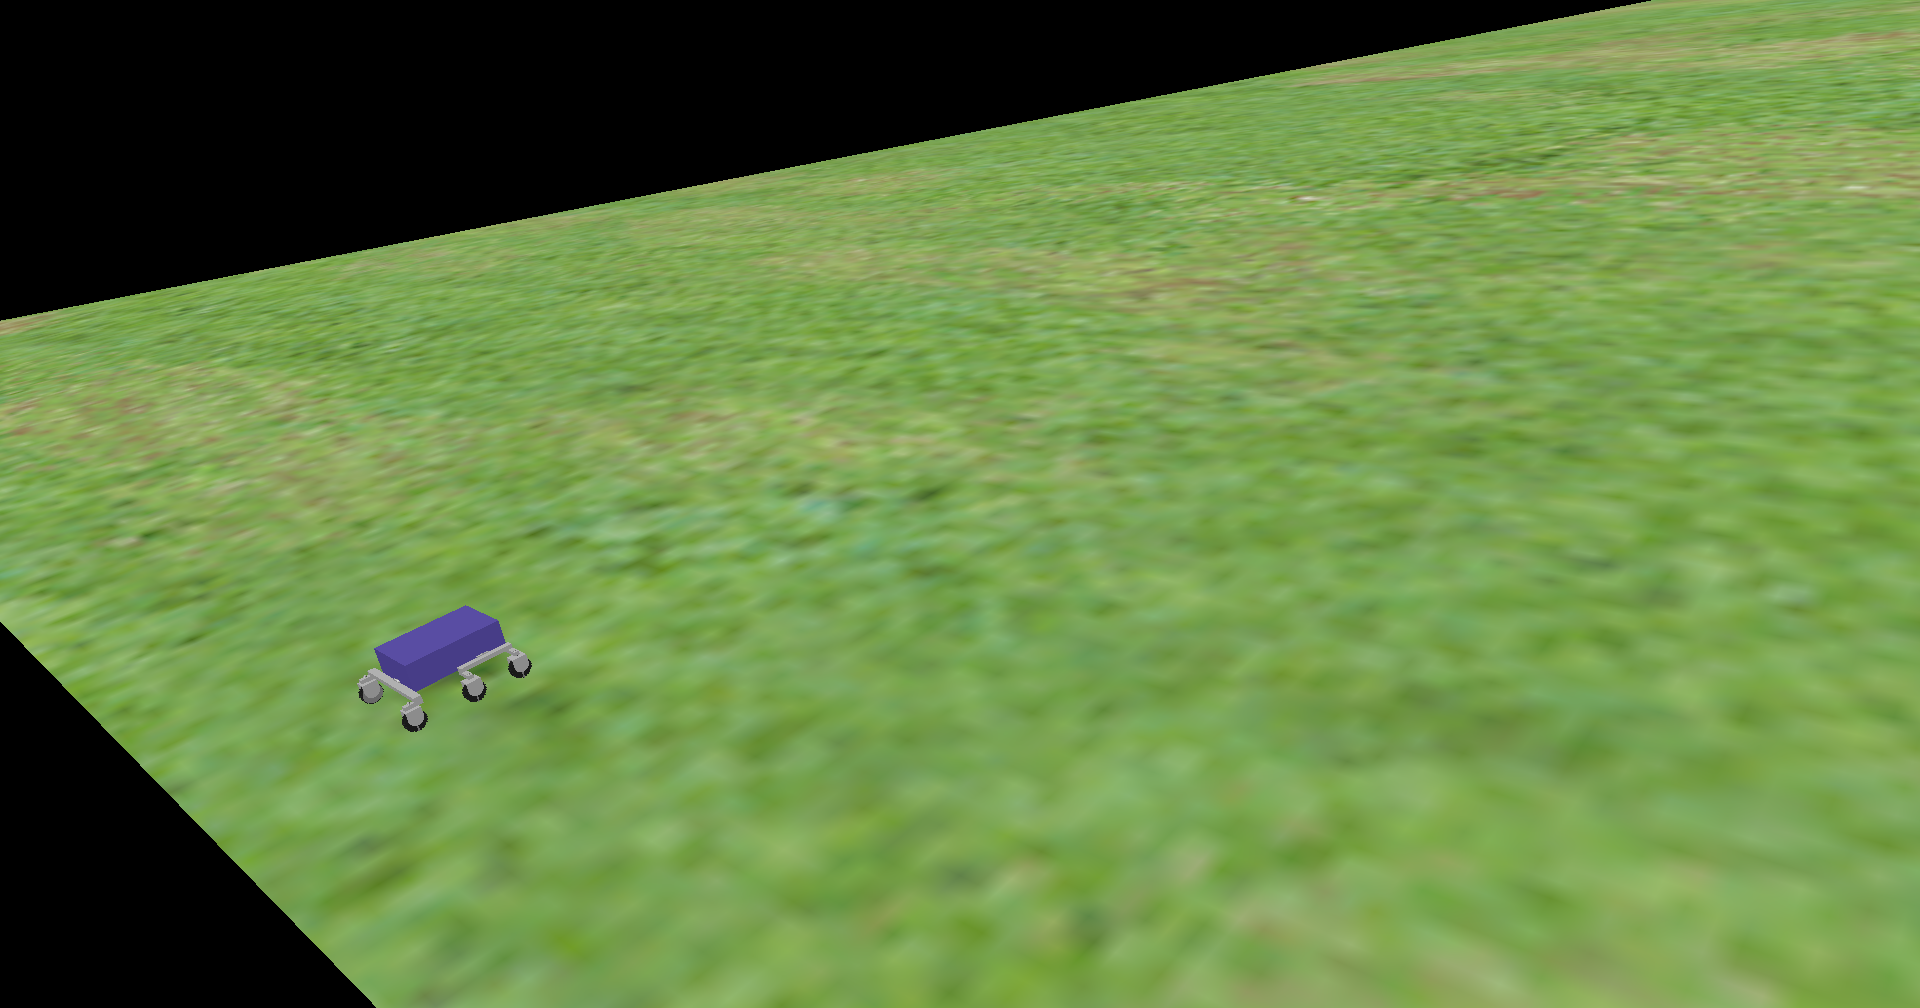
\includegraphics[width=0.8\textwidth]{run_4}
  \caption{Fourth test scenario}
\end{figure}

\noindent Rover's parcour has been devided into two phases:

\begin{enumerate} 
  \item $0s < t_s < 100s$, $\tau = 7495N$           
  \item $100s < t_s < 200s$, $\tau = 10000N$        
\end{enumerate}

\noindent In this case, following quantities have been plotted:

\begin{itemize}
  \item $x_{COM}$ - mass center coordinates
\end{itemize}

\begin{figure}[H]
  \centering
    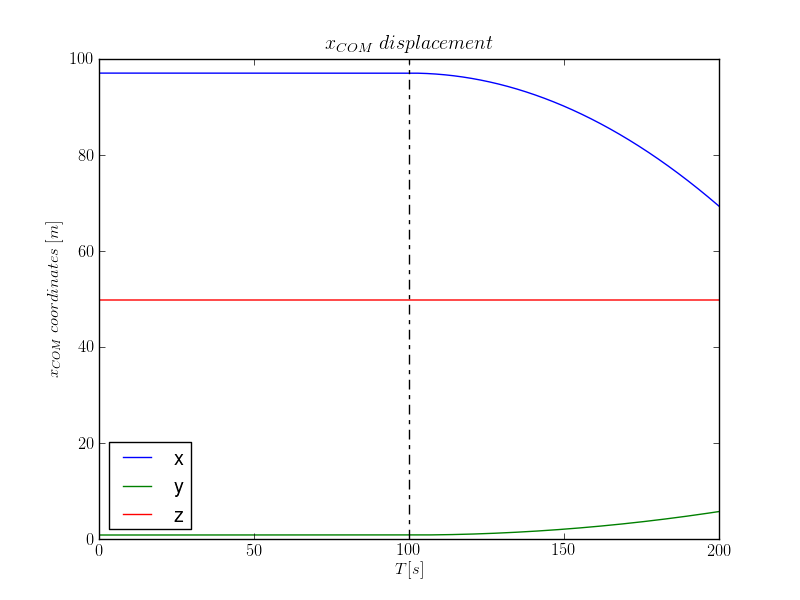
\includegraphics[width=0.8\textwidth]{xCOM4}
  \caption{$x_{COM}$}
\end{figure}

\begin{itemize}
  \item $x_{wheels}$ - wheels angular displacement 
\end{itemize}

\begin{figure}[H]
  \centering
    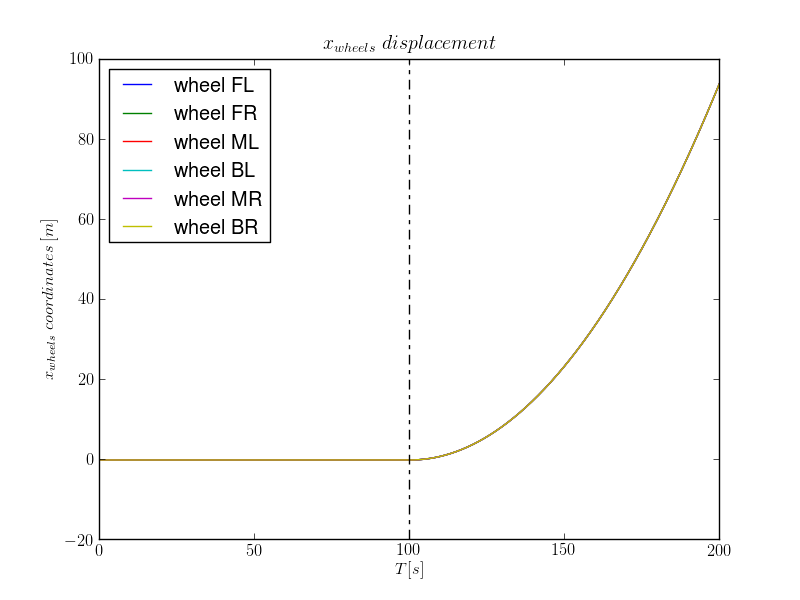
\includegraphics[width=0.8\textwidth]{xWHEELS4}
  \caption{$x_{wheels}$}
\end{figure}

\begin{itemize}
  \item $v_{COM}$ - mass center velocity
\end{itemize}

\begin{figure}[H]
  \centering
    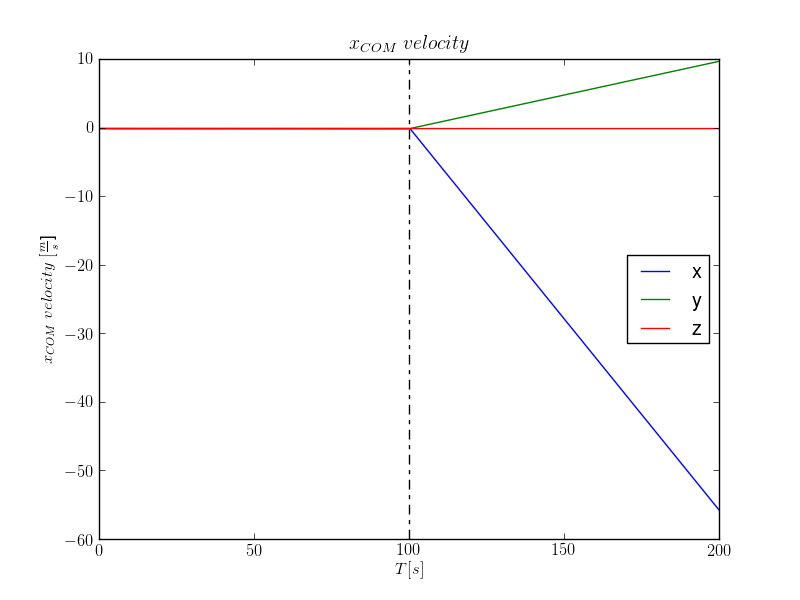
\includegraphics[width=0.8\textwidth]{vCOM4}
  \caption{$v_{COM}$}
\end{figure}

\begin{itemize}
  \item $v_{wheels}$ - wheels angular velocity
\end{itemize}

\begin{figure}[H]
  \centering
    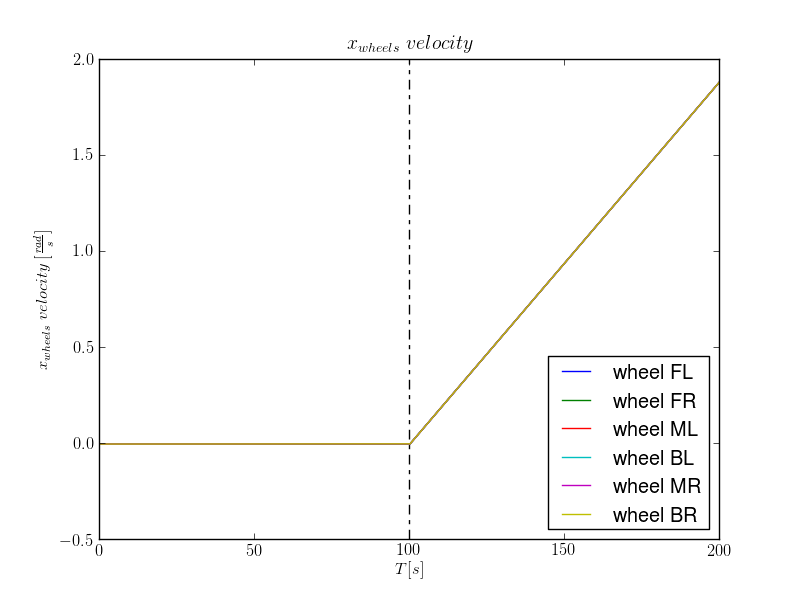
\includegraphics[width=0.8\textwidth]{vWHEELS4}
  \caption{$v_{wheels}$}
\end{figure}

\begin{itemize}
  \item $R_{COM}$ - reaction forces of center of mass in lagrangian coordinates
\end{itemize}

\begin{figure}[H]
  \centering
    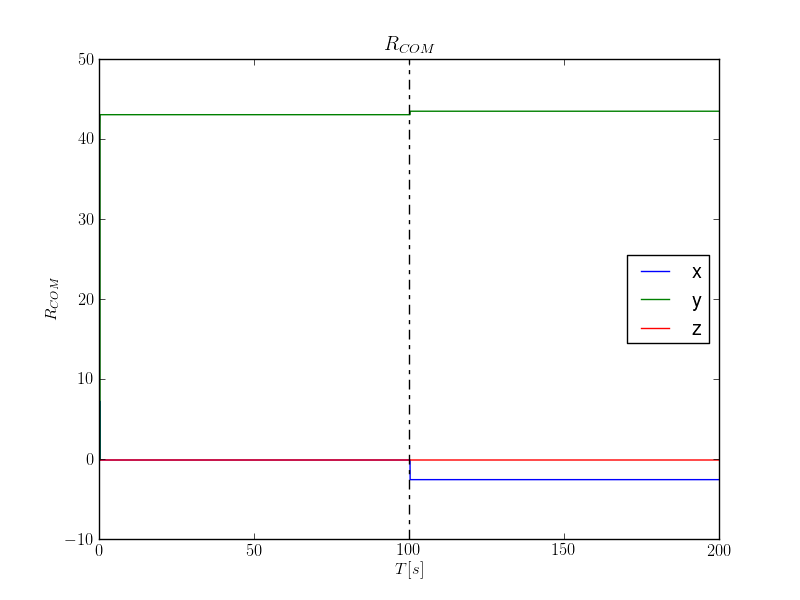
\includegraphics[width=0.8\textwidth]{pCOM4}
  \caption{$R_{COM}$}
\end{figure}

\begin{itemize}
  \item $R_{wheels}$ - reaction forces of wheels in lagrangian coordinates
\end{itemize}

\begin{figure}[H]
  \centering
    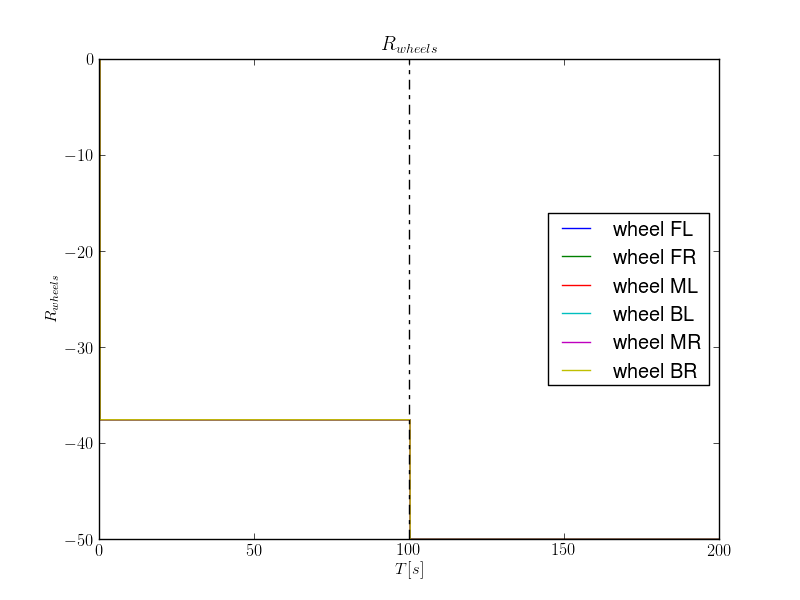
\includegraphics[width=0.8\textwidth]{pWHEELS4}
  \caption{$R_{wheels}$}
\end{figure}

\begin{itemize}
  \item $\lambda_{N}$ - normal component of the contact force (impulsion) for each wheel
\end{itemize}

\begin{figure}[H]
  \centering
    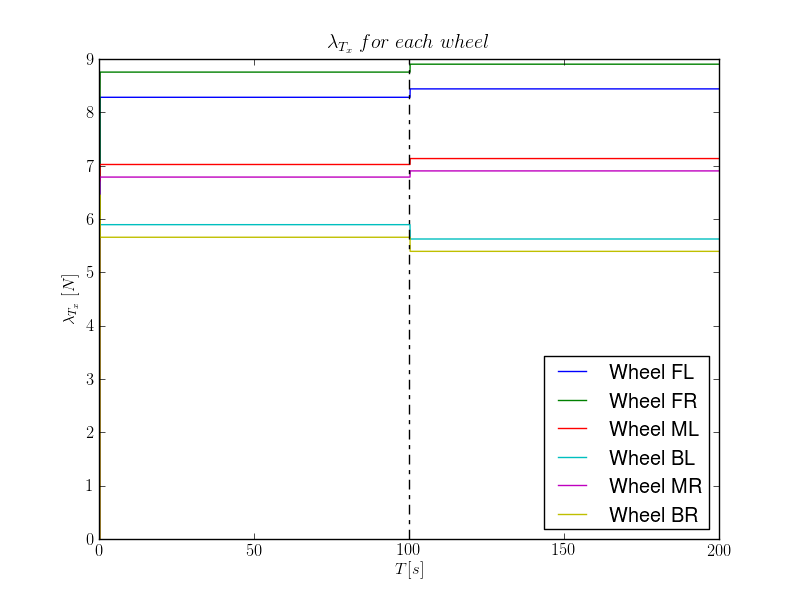
\includegraphics[width=0.8\textwidth]{lambdaN4}
  \caption{$\lambda_N$}
\end{figure}

\begin{itemize}
  \item $\lambda_{T_x}$ - tangential component of the contact force in the x direction for each wheel
\end{itemize}

\begin{figure}[H]
  \centering
    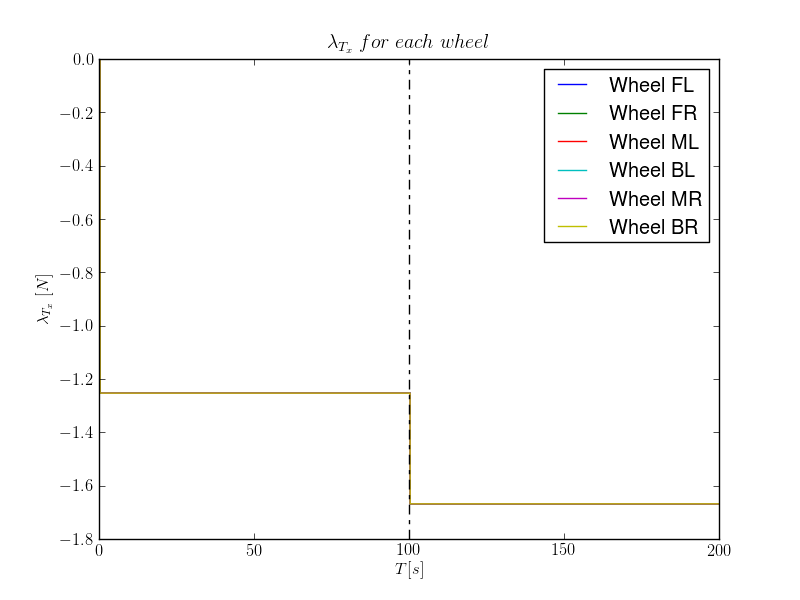
\includegraphics[width=0.8\textwidth]{lambdaTx4}
  \caption{$\lambda_{T_x}$}
\end{figure}

\begin{itemize}
  \item $\lambda_{T_z}$ - tangential component of the contact force in the z direction for each wheel
\end{itemize}

\begin{figure}[H]
  \centering
    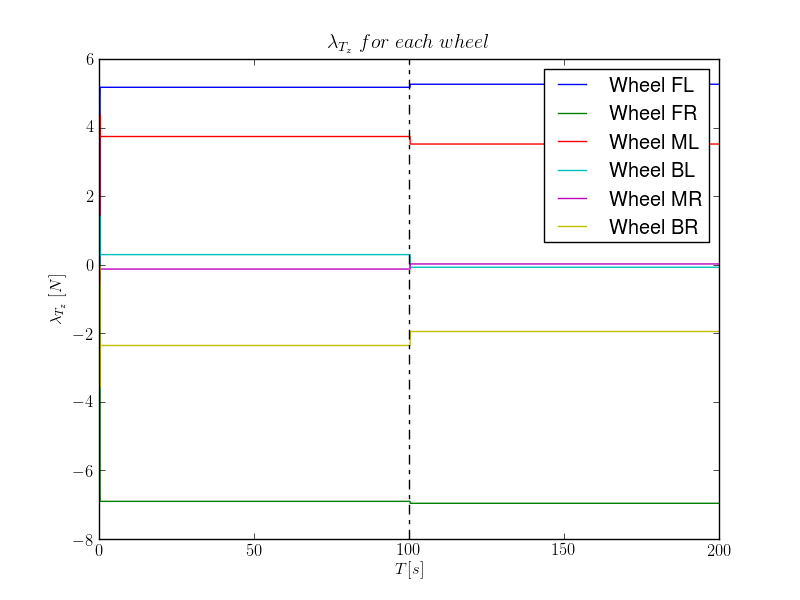
\includegraphics[width=0.8\textwidth]{lambdaTz4}
  \caption{$\lambda_{T_z}$}
\end{figure}

\begin{itemize}
  \item $y_{N}$ - gap function (distance between contact point and the constraint function) for each wheel
\end{itemize}

\begin{figure}[H]
  \centering
    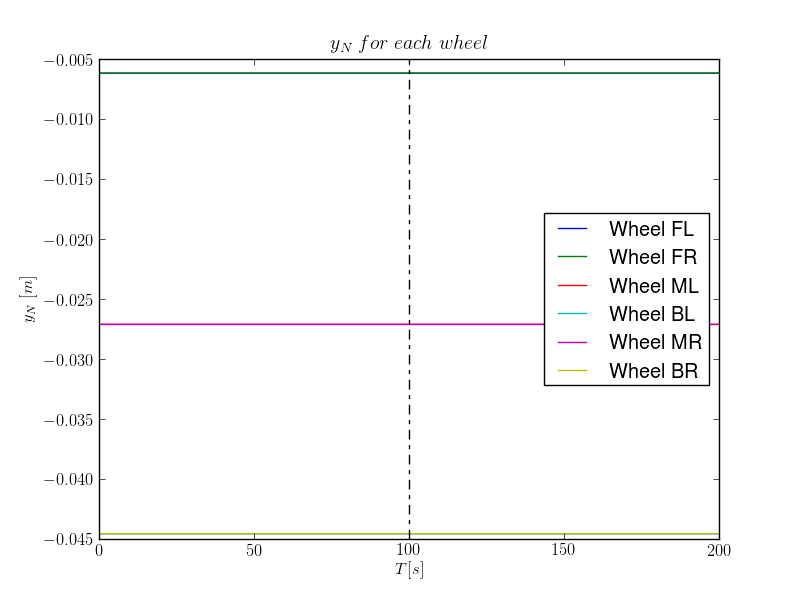
\includegraphics[width=0.8\textwidth]{yN4}
  \caption{$y_N$}
\end{figure}

\begin{itemize}
  \item $\dot{y}_{N}$ - normal component of the local contact velocity for each wheel
\end{itemize}

\begin{figure}[H]
  \centering
    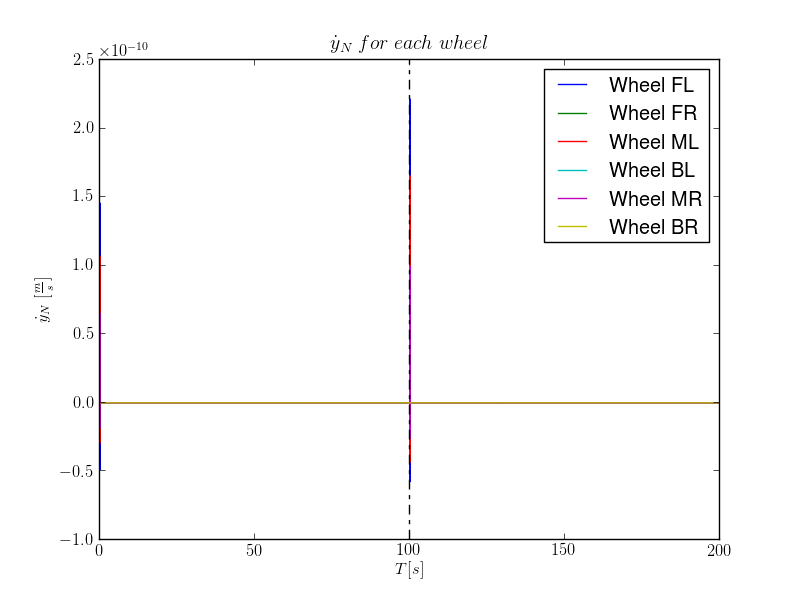
\includegraphics[width=0.8\textwidth]{yNdot4}
  \caption{$\dot{y}_{N}$}
\end{figure}

\begin{itemize}
  \item $\dot{y}_{T_x}$ - tangential component x of the local contact velocity for each wheel
\end{itemize}

\begin{figure}[H]
  \centering
    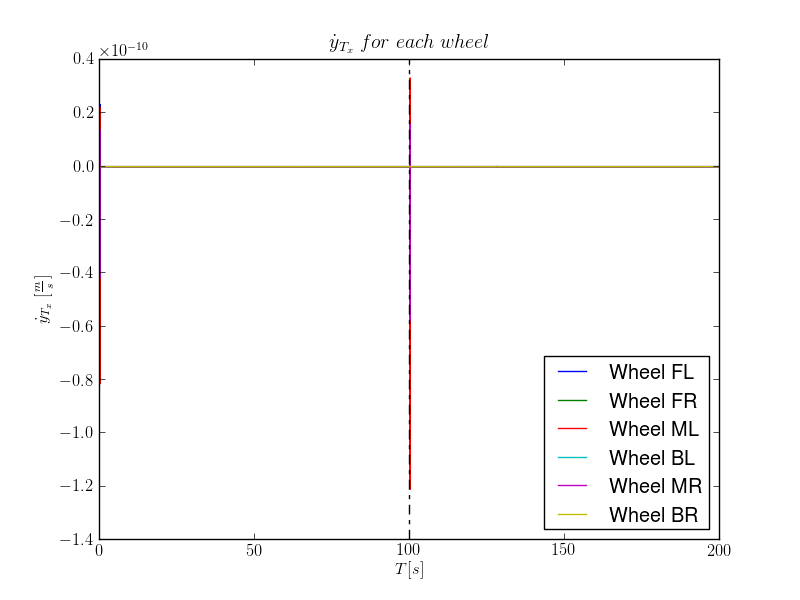
\includegraphics[width=0.8\textwidth]{yTxdots4}
  \caption{$\dot{y}_{T_x}$}
\end{figure}

\begin{itemize}
  \item $\dot{y}_{T_z}$ - tangential component z of the local contact velocity for each wheel
\end{itemize}

\begin{figure}[H]
  \centering
    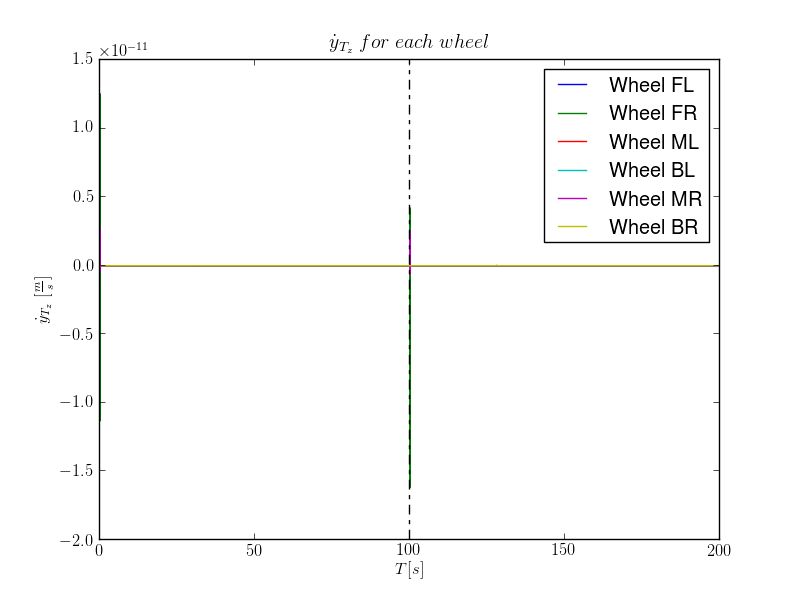
\includegraphics[width=0.8\textwidth]{yTzdots4}
  \caption{$\dot{y}_{T_z}$}
\end{figure}

